\documentclass[12pt, a4paper]{article}

\usepackage[hmargin=2.5cm, vmargin=2cm]{geometry}
\usepackage{amsthm, amssymb, mathtools, yhmath, graphicx}
\usepackage{fontspec, type1cm, titlesec, titling, fancyhdr, tabularx}
\usepackage{caption}
\usepackage{color}
\usepackage{hhline}
\usepackage{unicode-math}
\usepackage{nicefrac}
\usepackage[abbreviations]{siunitx}
\usepackage{comment}

\usepackage[CheckSingle, CJKmath]{xeCJK}
\usepackage{CJKulem}
\usepackage{enumitem}
\usepackage[usenames, dvipsnames]{xcolor}
\usepackage{colortbl}
\usepackage{circuitikz}
%\setCJKmainfont[BoldFont=cwTex Q Hei]{cwTex Q Ming}
%\setCJKsansfont[BoldFont=cwTex Q Hei]{cwTex Q Ming}
%\setCJKmonofont[BoldFont=cwTex Q Hei]{cwTex Q Ming}
\setCJKmainfont[BoldFont=cwTeX Q Hei]{cwTeX Q Ming}

\def\normalsize{\fontsize{12}{18}\selectfont}
\def\large{\fontsize{14}{21}\selectfont}
\def\Large{\fontsize{16}{24}\selectfont}
\def\LARGE{\fontsize{18}{27}\selectfont}
\def\Huge{\fontsize{20}{30}\selectfont}

\titleformat{\section}{\bf\Large}{\arabic{section}}{24pt}{}
\titleformat{\subsection}{\large}{\arabic{subsection}.}{12pt}{}
\titlespacing*{\subsection}{0pt}{0pt}{1.5ex}

\parindent=24pt

\DeclarePairedDelimiter{\abs}{\lvert}{\rvert}
\DeclarePairedDelimiter{\norm}{\lVert}{\rVert}
\DeclarePairedDelimiter{\inpd}{\langle}{\rangle}
\DeclarePairedDelimiter{\ceil}{\lceil}{\rceil}
\DeclarePairedDelimiter{\floor}{\lfloor}{\rfloor}

\newcommand{\unit}[1]{\:(\text{#1})}
\newcommand{\img}{\mathsf{i}}
\newcommand{\ex}{\mathsf{e}}
\newcommand{\dD}{\mathrm{d}}
\newcommand{\dI}{\,\mathrm{d}}
\DeclareSIUnit \uF {\micro \farad}
\DeclareSIUnit \mH {\milli \henry}

\title{ \bf {\huge 電子電路實驗6:RCL 電路之步級響應}\\ 實驗預報}
\author{B02901178 江誠敏}
\date{2014/09/21}

\begin{document}

\maketitle

\section{實驗目的}
本實驗將研究 RCL 二次線性電路的步級響應。
\section{實驗步驟}
\begin{enumerate}[itemsep=0pt]
  \item 利用 LCR 計,記錄所使用的各個電容以及電感的確實量值。
  \item 連接電路如圖 6.3,其中 L =10 mH,C = 0.01μF,R = 1kΩ,v 為低電位差−5V, 高電位差 5V,頻率 1kHz 之方波。
  \item 利用示波器觀察並記錄 vC、vL、vR的波形。
  \item 將 R 值改為 4kΩ,重複步驟 3。
  \item 嘗試調整 R 值(在 1kΩ至 4kΩ之間),使得示波器觀察到的圖形如臨界阻尼的情況(參考圖 6.2,即剛好快要開始有欠阻尼震盪的位置),並記錄此時 vC、vL、vR的波形。
  \item 量測臨界阻尼時的 R 值。
\end{enumerate}


  \begin{center}
    \begin{tikzpicture}[american voltages, scale=0.8]
      \draw[color=black, thick]
      (0, 0) to [V=$V_S$] (0, 6) 
      (0, 6) to [L, l=$L$, v=$V_L$] (6, 6) 
      (6, 6) to [R, l=$R$, v=$V_R$] (6, 0)
      (6, 0) to [C, l=$C$, v=$V_C$] (0, 0)
      (0, 0) node[ground]{}
      ;
    \end{tikzpicture}
  \end{center}


  \section{預報問題}

  \begin{enumerate}[itemsep=20pt, topsep=10pt]
    \item {\large\bf 請推導實驗原理中二次電路步級響應各個參數與各元件值之間的關係。} \\[10pt]
      假設步級響應指的是input為$u(t)$的反應。
      因此我們可以列出微分方程:
      \[
        L\frac{\dD I}{\dD t} + RI + \frac{1}{C} \int I \dI t = u(t)
      \]
      兩邊微分
      \[
        L\frac{\dD^2 I}{\dD t^2} + R\frac{\dD I}{\dD t} + \frac{1}{C} I = \delta(t)
      \]
      而在$t > 0, \delta(t) = 0$
      令
      \[
        \alpha_{1, 2} = -\frac{R}{2L} \pm \sqrt{ \left( \frac{R}{2L} \right)^2 - \frac{1}{LC} } 
      \]
      當$\alpha_1 \neq \alpha_2$時,微分方程有解
      \[
        I = A_1 \ex^{\alpha_1 t} + A_2 \ex^{\alpha_2 t}
      \]
      而$\alpha_1 = \alpha_2 = \alpha$時,
      \[
        I = A_1 \ex^{\alpha t} + A_2 t \ex^{\alpha t}
      \]
      初始條件則是$I(0+) = I(0-) = 0$,因為通過電感的電流需連續。且
      \[
        L \frac{\dD I}{\dD t} = V_L = V - V_R - V_C = V - I(0+)R - V(0+) = V - 0 - 0 = V
      \]
      因為電容的電壓需連續。由這兩個條件我們可以得出$A_1, A_2$。
    \item {\large\bf 在這個實驗中的二次電路,R 的理論值為多少時會造成臨界阻尼?} \\[10pt]
      臨界阻尼時
      \[
        \left( \frac{R}{2L} \right)^2 - \frac{1}{LC} = 0 \Leftrightarrow R = \sqrt{\frac{4L}{C}}
      \]
      因此如果$C = \SI{0.1}\uF, L = \SI{10}\mH$, 
      \[ R_0 = \frac{4 \cdot \SI{10}\mH}{\SI{0.01}\uF} = \SI{2}\kohm \]
    \item {\large\bf 請使用PSpice或者其他電路模擬軟體模擬實驗中使用的二次電路。請注意二次電路調整R至臨界阻尼的部分請用預報問題2的值。} \\[10pt]

      \begin{itemize}
        \item $R = \SI{1}\kohm$
      \begin{center}
        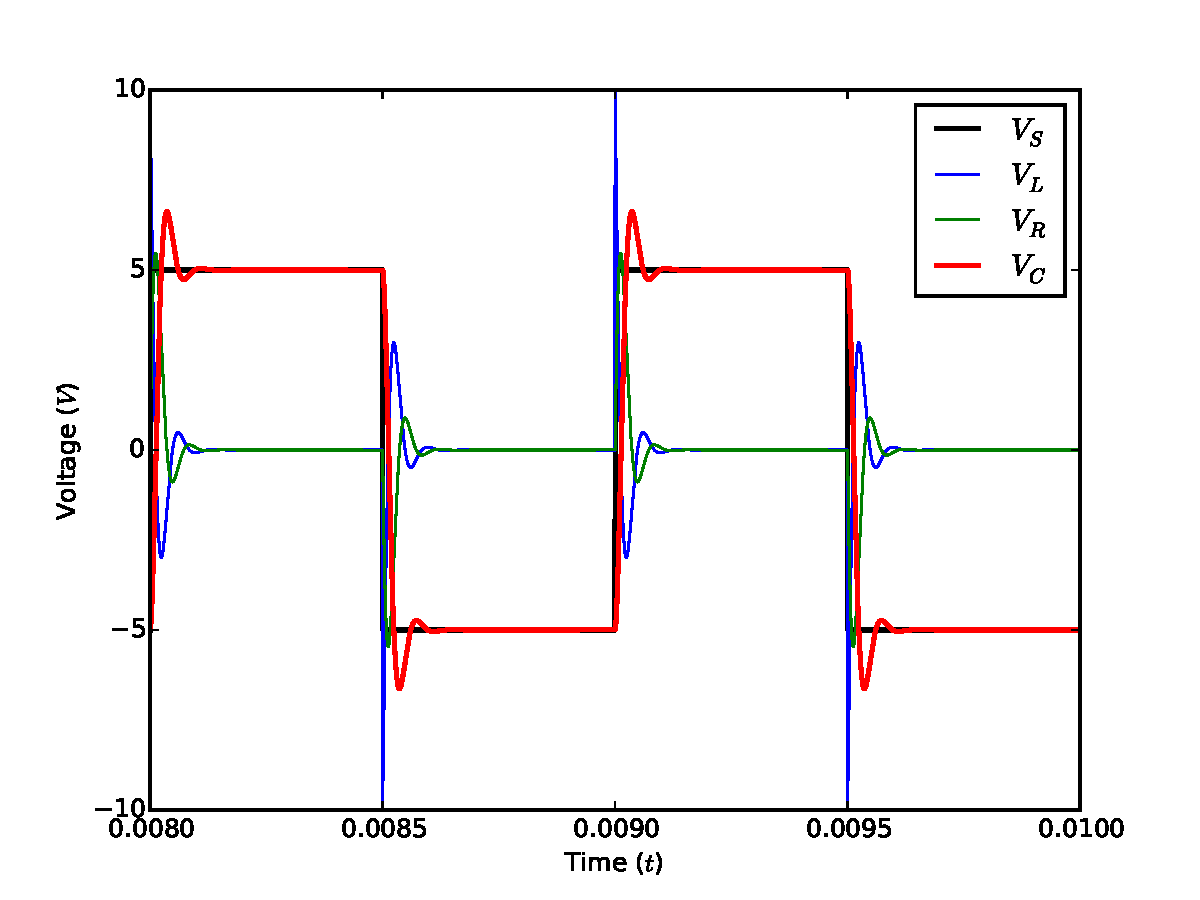
\includegraphics[width=0.6\textwidth]{data/plt1.pdf}
      \end{center}
        \item $R = \SI{4}\kohm$
      \begin{center}
        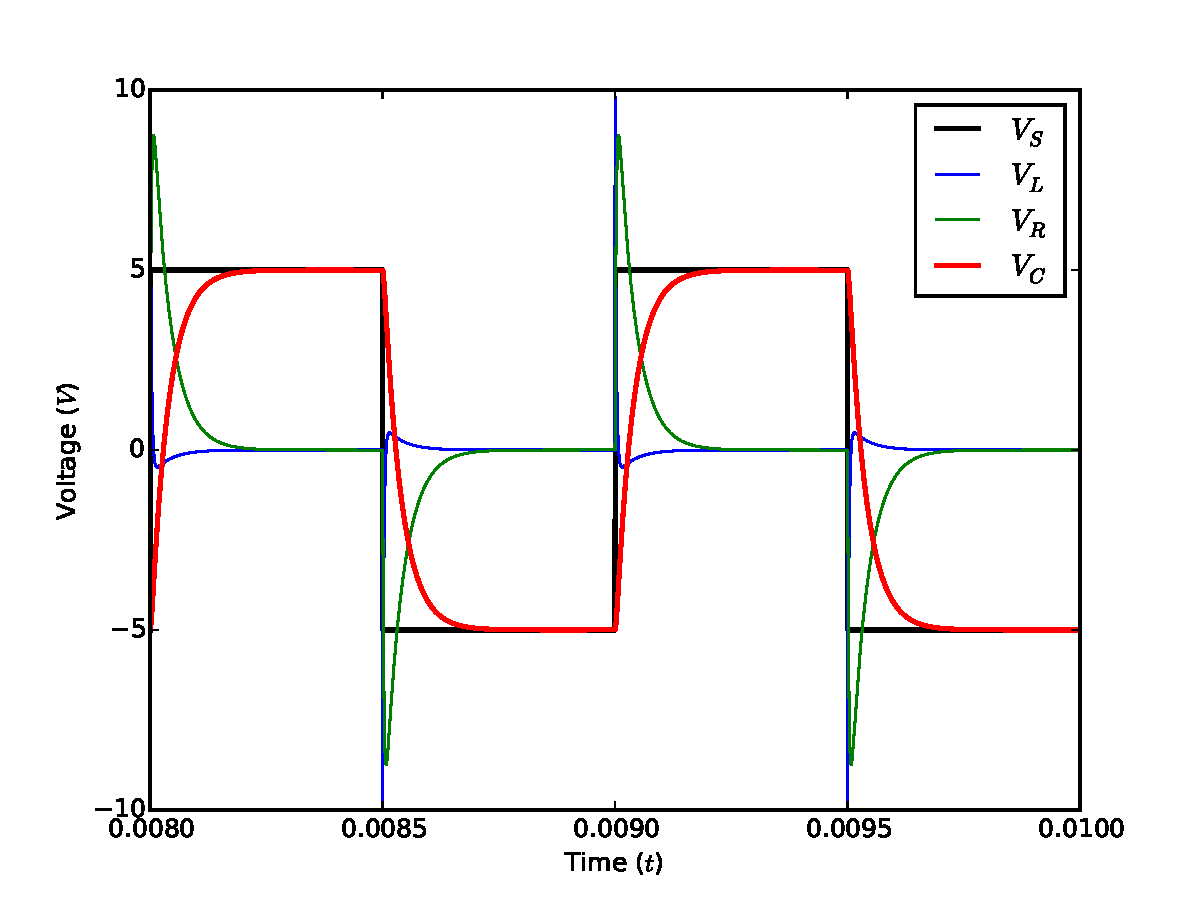
\includegraphics[width=0.6\textwidth]{data/plt3.pdf}
      \end{center}
        \item 臨界阻尼$R = \SI{2}\kohm$
      \begin{center}
        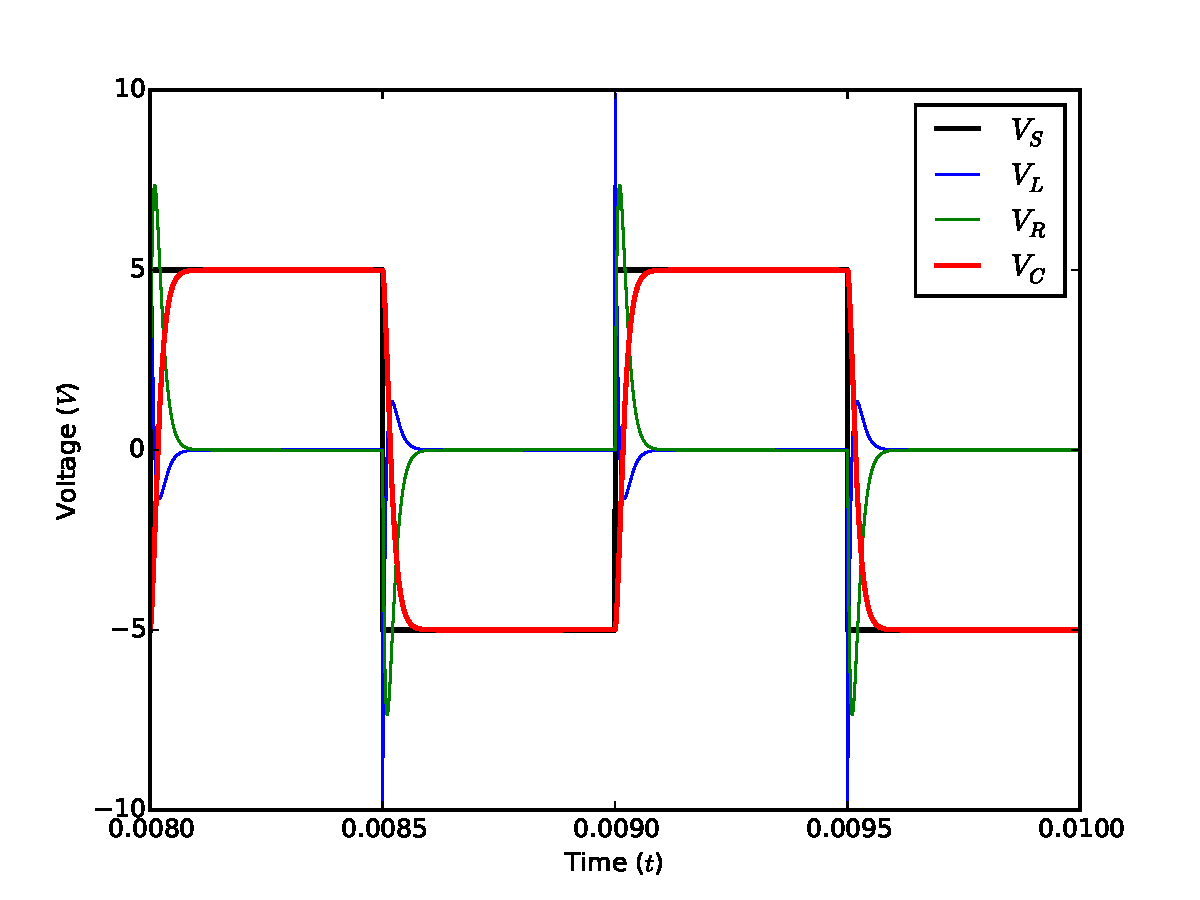
\includegraphics[width=0.6\textwidth]{data/plt2.pdf}
      \end{center}
  \end{itemize}
  
  \end{enumerate}

\end{document}


